%credits K. Κουνής, I. Στεφανίδου 
%refactoring : K.Draziotis (drazioti@gmail.com)
%Licence CC_BY_SA

\documentclass[12pt]{article}
\usepackage{helvet} 
\usepackage{amsmath}
\usepackage{titlesec}
\usepackage{lipsum}
\usepackage{graphicx}
\graphicspath{{images/}}


\usepackage{listings}
\usepackage{xcolor}

\definecolor{codegreen}{rgb}{0,0.6,0}
\definecolor{codegray}{rgb}{0.5,0.5,0.5}
\definecolor{codepurple}{rgb}{0.58,0,0.82}
\definecolor{backcolour}{rgb}{0.95,0.95,0.92}

\lstdefinestyle{mystyle}{
	backgroundcolor=\color{backcolour},   
	commentstyle=\color{codegreen},
	keywordstyle=\color{magenta},
	numberstyle=\tiny\color{codegray},
	stringstyle=\color{codepurple},
	basicstyle=\ttfamily\footnotesize,
	breakatwhitespace=false,         
	breaklines=true,                 
	captionpos=b,                    
	keepspaces=true,                 
	numbers=left,                    
	numbersep=5pt,                  
	showspaces=false,                
	showstringspaces=false,
	showtabs=false,                  
	tabsize=2
}
\lstset{style=mystyle}

\titleformat{\section}[display]
{\clearpage\vspace*{50pt}%
	\normalfont\huge\bfseries}%
{{\Kappa}E{\Phi}A{\Lambda}AIO \thesection}%
{20pt}%
{\Huge}%
[\vspace{40pt}]

\usepackage[algosection,commentsnumbered,ruled,vlined]{algorithm2e}
\NoCaptionOfAlgo
\usepackage{chemarrow}
\newcommand\aug{\fboxsep=-\fboxrule\!\!\!\fbox{\strut}\!\!\!}
\usepackage{graphicx}
\usepackage{gfsdidot}
\usepackage[LGR,T1]{fontenc}
\usepackage[utf8]{inputenc}
\usepackage[english,greek]{babel} % και για τις δυο γλώσσες
\usepackage{alphabeta}
\usepackage[hidelinks]{hyperref}
\usepackage{hyperref}
\usepackage{makeidx}
\usepackage{enumerate}
\usepackage{enumitem}
\usepackage{systeme}
\usepackage{algorithmic}
\usepackage{comment}

% TEXT FORMATTING
% set spacing between lines (διάστιχο)
\usepackage{setspace}
\setstretch{1.5}
% package to customize chapters, sections and subsections style
\usepackage{titlesec}
% chapter title appearance format
\titleformat{\chapter}[display]
{\bfseries\huge}{\chaptertitlename\space\thechapter}{16pt}{}
% https://www.sharelatex.com/learn/Sections_and_chapters
\titlespacing{\chapter}{0pc}{1.5ex plus .1ex minus .2ex}{5pc}
% section title appearance format
\titleformat{\section}
{\bfseries\large}{\thesection}{14pt}{}
% subsection title appearance format
\titleformat{\subsection}
{\bfseries\normalsize}{\thesubsection}{12pt}{}
% set margins
\usepackage{geometry}
\geometry{left=3cm, right=2cm, top=4cm, bottom=3cm}
\usepackage{graphicx}
% put images in images path
\graphicspath{{images/}}
\usepackage{setspace}

% Caption customization
% use this package to set appearance for captions
\usepackage{caption}
% caption size for figures 10pt
\captionsetup[figure]{font=footnotesize,labelfont=footnotesize}
% caption size for tables 10pt and underlined
\usepackage[normalem]{ulem} % Package for underlining
\DeclareCaptionLabelFormat{label_format}{\uline{#1~#2}} % underline label
\DeclareCaptionTextFormat{text_format}{\uline{#1}} % underline text
\DeclareCaptionLabelSeparator{separator_format}{\uline{:~}} % underline separator
\captionsetup[table]{font=normalsize,labelfont=normalsize,labelformat=label_format,textformat=text_format,labelseparator=separator_format}

% use this package to define custom colors
\usepackage{xcolor}

% create colors
\colorlet{punct}{red!60!black}
\definecolor{background}{HTML}{EEEEEE}
\definecolor{delim}{RGB}{20,105,176}
\colorlet{numb}{magenta!60!black}


\usepackage{amsfonts}
\usepackage{amscd}
\usepackage{amssymb}
\newtheorem{algor}{\bf{Algorithm}}[subsection]


\newtheorem{remark}{Remark}[section]

\newtheorem{theorem}{Theorem}[section]
\newtheorem{lemma}[theorem]{Lemma}
%\newtheorem{corollary}[theorem]{Corollary}
\newtheorem{definition}[theorem]{Definition}
\newtheorem{proposition}[theorem]{Proposition}
%\theoremstyle{remark}
%\newtheorem{example}[theorem]{Example}
%\newtheorem{remark}[theorem]{Remark}
\numberwithin{equation}{section}

% use this package to show actual code listings
\usepackage{listings}

% change listings name in caption to Απεικόνιση
\renewcommand{\lstlistingname}{Απεικόνιση}

% change listings name in contents page to Κατάλογος απεικονήσεων
\renewcommand\lstlistlistingname{Κατάλογος απεικονίσεων}

% set custom colorscheme for listings with language=lang1 to make them stand out more
% http://tex.stackexchange.com/questions/83085/how-to-improve-listings-display-of-json-files
\lstdefinelanguage{lang1}{
	basicstyle=\normalfont\ttfamily,
	%    numbers=left,
	%    numberstyle=\scriptsize,
	%    stepnumber=1,
	%    numbersep=8pt,
	showstringspaces=false,
	breaklines=true,
	frame=lines,
	backgroundcolor=\color{background},
	literate=
	*{0}{{{\color{numb}0}}}{1}
	{1}{{{\color{numb}1}}}{1}
	{2}{{{\color{numb}2}}}{1}
	{3}{{{\color{numb}3}}}{1}
	{4}{{{\color{numb}4}}}{1}
	{5}{{{\color{numb}5}}}{1}
	{6}{{{\color{numb}6}}}{1}
	{7}{{{\color{numb}7}}}{1}
	{8}{{{\color{numb}8}}}{1}
	{9}{{{\color{numb}9}}}{1}
	{:}{{{\color{punct}{:}}}}{1}
	{,}{{{\color{punct}{,}}}}{1}
	{\{}{{{\color{delim}{\{}}}}{1}
	{\}}{{{\color{delim}{\}}}}}{1}
	{[}{{{\color{delim}{[}}}}{1}
	{]}{{{\color{delim}{]}}}}{1},
}


% create command for blank page
\usepackage{afterpage}
\newcommand\blankpage{%
	\null
	\thispagestyle{empty}%
	\addtocounter{page}{-1}%
	\newpage}

\definecolor{maroon}{HTML}{AF3235}
% add clickable hyperlinks
\usepackage{hyperref}
\hypersetup{
	colorlinks,
	citecolor=black,
	filecolor=black,
	linkcolor=black,
	urlcolor=black
}

% use fancy header and footer
\usepackage{fancyhdr}
\usepackage{blindtext} % to quickly get a full document

% Turn on the style
\pagestyle{fancy}

% Clear the header and footer
\fancyhf{}

% Set the right side of the footer to be the page number
\fancyfoot[R]{\thepage}

% set page number appearance to bottom right
\fancypagestyle{plain}{%
	\renewcommand{\headrulewidth}{0pt}
	\fancyhf{}
	\fancyfoot[R]{\thepage}%
}

\newcommand{\HRule}{\rule{\linewidth}{0.5mm}}
\newcommand{\lt}{\latintext}

\begin{document}
	\begin{titlepage}
		
		{\LARGE Αριστοτέλειο Πανεπιστήμιο Θεσσαλονίκης}
		\begin{center} {\Large Σχολή Θετικών Επιστημών} \end{center}
		\begin{figure}[h]
			\raggedright
			\hspace{90pt}
			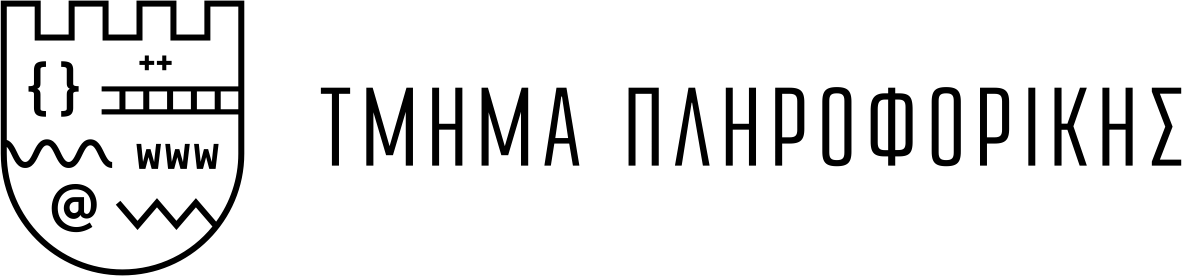
\includegraphics[width=0.5\linewidth]{logo.png}
		\end{figure}
		\begin{center}
			
			
			\begin{figure}[h]
				\centering 
				%\includegraphics[width=0.3\linewidth]{authLogo.png}
			\end{figure}
			\begin{center}
				% leave 2 cm from above text
				
				\HRule \\[0.4cm]
				{\huge Εργασία στο μάθημα της Κρυπτογραφίας}
				
				\HRule \\[0.4cm]
			\end{center}
			
			% put this on the bottom
			\vfill
			\begin{doublespacing}
				
				{\LARGE 
					Φτιάκας Σωτήριος ΑΕΜ: 3076\\}
				{\LARGE 
					Μπάρμπας Γρηγόριος ΑΕΜ: 3108\\}
				
				
				\vfill 
				{\Large \today}
			\end{doublespacing}
		\end{center}
	\end{titlepage}
	
	
	% insert table of contents
	\tableofcontents
	
	\clearpage
	
	
	\addcontentsline{toc}{section}{Περίληψη}
	\section*{{\color{maroon}Περίληψη}}
	
	..............
	% leave blank page before main part
	\blankpage
	
	\addcontentsline{toc}{section}{Θέμα 1}
	\section*{{\color{maroon}Θέμα 1}}
	
	\addcontentsline{toc}{section}{Θέμα 2}
	\section*{{\color{maroon}Θέμα 2}}
	
	\addcontentsline{toc}{section}{Θέμα 3}
	\section*{{\color{maroon}Θέμα 3}}
	
	\addcontentsline{toc}{section}{Θέμα 4}
	\section*{{\color{maroon}Θέμα 4}}
	
	\addcontentsline{toc}{section}{Θέμα 5}
	\section*{{\color{maroon}Θέμα 5}}
	
	\section*{\lt{Dictionary Attack}}
	
	{\lt{
			\lstinputlisting[language=python]{Code/No5.py}
	}}
	
	\addcontentsline{toc}{section}{Θέμα 6}
	\section*{{\color{maroon}Θέμα 6}}
	
	\addcontentsline{toc}{section}{Θέμα 7}
	\section*{{\color{maroon}Θέμα 7}}
	
	\section*{\lt{Shift Operator with XOR}}
	
	{\lt{
			m: 16-bits
			$$c=m\oplus(m<<6)\oplus(m<<10)$$
				
			Όπου $m<<a$ είναι κύλιση προς τα αριστερά κατά $a$-bits.
			
			Για μήνυμα $m$ και κλειδί $k$ ισχύει:
			Αν $c = m \oplus k$, τότε $m = c \oplus k$ 
				
			Επιπλέον, στην αρχική μας συνάρτηση κρυπτογράφησης, μπορούμε να κυλίσουμε και τα δύο μέλη ταυτόχρονα.
			$$(c<<2) = (m\oplus(m<<6)\oplus(m<<10))<<2$$
			
			$$\Leftrightarrow (c<<2) = (m<<2)\oplus(m<<8)\oplus(m<<12)$$
				
			Σημείωση: το $x<<i$ θα συμβολίζεται ως $x_i$ για ευκολία. \newline
			Συνεπώς θα έχουμε:	
			\begin{gather*} 
			c_0 = m_0 \oplus m_6 \oplus m_{10} \quad (1) \\
			c_2 = m_2 \oplus m_8 \oplus m_{12} \Rightarrow m_8 = m_2 \oplus m_{12} \oplus c_2 \quad (4) \\
			c_4 = m_4 \oplus m_{10} \oplus m_{14} \Rightarrow m_{10} = m_4 \oplus m_{14} \oplus c_4 \quad (2) \\
			c_6 = m_6 \oplus m_{12} \oplus m_0 \quad (5) \\
			c_8 = m_8 \oplus m_{14} \oplus m_2 \\
			c_{10} = m_{10} \oplus m_0 \oplus m_4 \\
			c_{12} = m_{12} \oplus m_2 \oplus m_6 \\
			c_{14} = m_{14} \oplus m_4 \oplus m_8 \Rightarrow m_{14} \oplus m_4 = m_8 \oplus c_{14} \quad (3) \\
			\end{gather*}
			
			Ξεκινώντας από την (1) έχουμε διαδοχικά:
			\begin{gather*} 
			c_0 = m_0 \oplus m_6 \oplus m_{10} \\ 
			(2)\Rightarrow c_0 = m_0 \oplus m_6 \oplus m_4 \oplus m_{14} \oplus c_4 \\
			(3)\Rightarrow c_0 \oplus c_4 = m_0 \oplus m_6 \oplus m_8 \oplus c_{14} \\
			(4)\Rightarrow c_0 \oplus c_4 \oplus c_{14} = m_0 \oplus m_6 \oplus m_2 \oplus m_{12} \oplus c_2 \\
			(5)\Rightarrow c_0 \oplus c_4 \oplus c_{14} \oplus c_2 = m_2 \oplus c_6 \\
			\Rightarrow c_0 \oplus c_4 \oplus c_{14} \oplus c_2 \oplus c_6 = m_2 \quad (6)
			\end{gather*}
			
			Κάνουμε κύλιση και στα δύο μέρη του (6) προς τα δεξιά και έχουμε:
			$$m_0 = c_{14} \oplus c_2 \oplus c_{12} \oplus c_0 \oplus c_4$$
			
			και άρα τελικά έχουμε: $$m_0 = c_0 \oplus c_2 \oplus c_4 \oplus c_{12} \oplus c_{14}$$
	}}
	Κώδικας σε \lt{python}
	{\lt{
			\lstinputlisting[language=python]{Code/No7.py}
	}}
	
	\addcontentsline{toc}{section}{Θέμα 8}
	\section*{{\color{maroon}Θέμα 8}}
	
	\addcontentsline{toc}{section}{Θέμα 9}
	\section*{{\color{maroon}Θέμα 9}}
	
	\section*{\lt{Entropy}}
	{\lt{
		\begin{table}[h!]
			\centering
			\begin{tabular}{|c|c|c|c|c|c|c|c|c|}
				\hline
				\textbf{Υ/X} & \textbf{0} & \textbf{1} & \textbf{2}\\
				\hline
				\textbf{0} & 1/7 & 1/7 & 1/7 \\
				\hline
				\textbf{1} & 0 & 1/7 & 1/7 \\
				\hline
				\textbf{2} & 2/7 & 0 & 0 \\
				\hline
			\end{tabular}
		\end{table}
		Αρχικά υπολογίζουμε
		\begin{gather*} 
			p_x(X=0) = \sum_{y}p_{X,Y}(0,y)=\frac{3}{7} \\
			p_x(X=1) = \sum_{y}p_{X,Y}(1,y)=\frac{2}{7} \\
			p_x(X=2) = \sum_{y}p_{X,Y}(2,y)=\frac{2}{7} \\
			p_y(Y=0) = \sum_{y}p_{X,Y}(x,0)=\frac{3}{7} \\
			p_y(Y=1) = \sum_{y}p_{X,Y}(x,1)=\frac{2}{7} \\
			p_y(Y=2) = \sum_{y}p_{X,Y}(x,2)=\frac{2}{7}
		\end{gather*}
		
		Ισχύει ότι:
		$$H(X) = -\sum_{x}p_{X}(x)\log _{2}p_{X}(x) $$
		
		Επομένως
		\begin{gather*} 
			H(X) = -\frac{3}{7}\log _{2}\frac{3}{7} - \frac{2}{7}\log _{2}\frac{2}{7} - \frac{2}{7}\log _{2}\frac{2}{7} \\
			= -\frac{3}{7}\log _{2}\frac{3}{7} -\frac{4}{7}\log _{2}\frac{2}{7} \\
			\simeq 1.5566567074628228\\
			\\		
			Υ(Χ) = -\frac{3}{7}\log _{2}\frac{3}{7} - \frac{2}{7}\log _{2}\frac{2}{7} - \frac{2}{7}\log _{2}\frac{2}{7} \\
			= -\frac{3}{7}\log _{2}\frac{3}{7} -\frac{4}{7}\log _{2}\frac{2}{7} \\
			\simeq 1.5566567074628228
		\end{gather*}
		
		Επίσης έχουμε τον εξής τύπο
		$$H(X,Y)=-\sum_{x}\sum_{y}p(x,y)\log_{2}p(x,y)$$
		Άρα θα έχουμε:
		\begin{gather*} 
			Η(X,Υ) = - p(0,0)\log_{2}p(0,0) - p(0,1)\log_{2}p(0,1) - p(0,2)\log_{2}p(0,2) - \\ p(1,0)\log_{2}p(1,0) - p(1,1)\log_{2}p(1,1) - p(1,2)\log_{2}p(1,2) - \\
			p(2,0)\log_{2}p(2,0) -  p(2,1)\log_{2}p(2,1) - p(2,2)\log_{2}p(2,2) \\
			\simeq 2.5216406363433186
		\end{gather*}
		
		Θα υπολογίσουμε την $H(Y|X)$.
		Χρειαζόμαστε αρχικά τα παρακάτω,
		\begin{gather*} 
			p_{Y|X}(y=0|x=0) = \frac{p_{X,Y}(0,0)}{p_{X}(0)} = \frac{\frac{1}{7}}{\frac{3}{7}} =\frac{1}{3} \\
			p_{Y|X}(y=1|x=0) = \frac{p_{X,Y}(0,1)}{p_{X}(0)} = \frac{0}{\frac{3}{7}} = 0 \\
			p_{Y|X}(y=2|x=0) = \frac{p_{X,Y}(0,2)}{p_{X}(0)} = \frac{\frac{2}{7}}{\frac{3}{7}} =\frac{2}{3} \\
			p_{Y|X}(y=0|x=1) = \frac{p_{X,Y}(1,0)}{p_{X}(1)} = \frac{\frac{1}{7}}{\frac{2}{7}} =\frac{1}{2} \\
			p_{Y|X}(y=1|x=1) = \frac{p_{X,Y}(1,1)}{p_{X}(1)} = \frac{\frac{1}{7}}{\frac{2}{7}} =\frac{1}{2} \\
			p_{Y|X}(y=2|x=1) = \frac{p_{X,Y}(1,2)}{p_{X}(1)} = \frac{0}{\frac{2}{7}} = 0 \\
			p_{Y|X}(y=0|x=2) = \frac{p_{X,Y}(2,0)}{p_{X}(2)} = \frac{\frac{1}{7}}{\frac{2}{7}} =\frac{1}{2} \\
			p_{Y|X}(y=1|x=2) = \frac{p_{X,Y}(2,1)}{p_{X}(2)} = \frac{\frac{1}{7}}{\frac{2}{7}} =\frac{1}{2} \\
			p_{Y|X}(y=2|x=2) = \frac{p_{X,Y}(2,2)}{p_{X}(2)} = \frac{0}{\frac{2}{7}} = 0
		\end{gather*}		
	}}

	Τώρα πρέπει να υπολογίσουμε τα παρακάτω: 
	\begin{gather*} 
		H(Y|X=0) = - \sum_{y}p_{Y|X}(y|x=0)\log_{2}p_{Y|X}(y|x=0) \\
		= -(\frac{1}{3}\log_{2}\frac{1}{3} + 0 + \frac{2}{3}\log_{2}\frac{2}{3}) \\
		= -(\frac{1}{3}\log_{2}\frac{1}{3} + \frac{2}{3}\log_{2}\frac{2}{3}) \\
		H(Y|X=1) = - \sum_{y}p_{Y|X}(y|x=1)\log_{2}p_{Y|X}(y|x=1) \\
		= -(\frac{1}{2}\log_{2}\frac{1}{2} + \frac{1}{2}\log_{2}\frac{1}{2} + 0) \\
		= - \log_{2}2 = 1\\
		H(Y|X=2) = - \sum_{y}p_{Y|X}(y|x=2)\log_{2}p_{Y|X}(y|x=2) \\
		= - \log_{2}2 = 1\\
	\end{gather*}
	
	Τότε θα έχουμε
	\begin{gather*} 
		H(Y|X) = \sum_{x}p_{X}xH(Y|X=x) \\
		= p_{X}(0)H(Y|X=0) + p_{X}(1)H(Y|X=1) + p_{x}(2)H(Y|X=2) \\
		\simeq 0.9649839288804954
	\end{gather*}
	
	Γνωρίζουμε επίσης ότι από το θεώρημα της αμοιβαίας πληροφορίας έχουμε
	$$I(X,Y) = H(X) - H(X|Y) = H(Y) - H(Y|X)$$
	
	Άρα έχουμε
	\begin{gather*} 
		H(X|Y) = -(H(Y) - H(Y|X) - H(X)) \\
		\simeq 0.9649839288804954 
	\end{gather*}
	
	Τέλος,
	\begin{gather*} 
		ρ = 1 - \frac{H(Y|X)}{H(X)} \\
		\simeq 0.5916727785823274
	\end{gather*}
	
	Κώδικας σε \lt{python}
	{\lt{
			\lstinputlisting[language=python]{Code/No9.py}
	}}
	
	\addcontentsline{toc}{section}{Θέμα 10}
	\section*{{\color{maroon}Θέμα 10}}
	
	\addcontentsline{toc}{section}{Θέμα 11}
	\section*{{\color{maroon}Θέμα 11}}
	
	\addcontentsline{toc}{section}{Θέμα 12}
	\section*{{\color{maroon}Θέμα 12}}
	
	\addcontentsline{toc}{section}{Θέμα 13}
	\section*{{\color{maroon}Θέμα 13}}
	
	\section*{\lt{Chinese Theorem}}
	{\lt{
			Έχουμε το σύστημα των γραμμικών ισοδυναμιών
			\begin{gather*} 
				x \equiv 9 \pmod{19} \\
				x \equiv 9 \pmod{12} \\
				x \equiv 13 \pmod{19}
			\end{gather*}
			
			Έχουμε ότι ισχύει $\gcd(12,17,19) = 1$, άρα δεν απαιτείται κάποια απλοποίηση.
			
			Για την επίλυση του συστήματος χρησιμοποιούμε το Κινέζικο Θεώρημα Υπολοίπων
			
			Έτσι έχουμε: $m=17*12*19=3876$
			
			\begin{gather*} 
				M_1 = 228y_1 \equiv 1 \mod{17} \implies 7y_1 \equiv \mod{17} \implies y_1=5 \\
				M_2 = 323y_2 \equiv 1 \mod{12} \implies 11y_1 \equiv \mod{12} \implies y_1=11 \\
				M_3 = 204y_3 \equiv 1 \mod{19} \implies 14y_1 \equiv \mod{19} \implies y_1=15
			\end{gather*}
			
			Τώρα πολλαπλασιάζουμε και προσθέτουμε:
			\begin{gather*}
				x = 9*228*5 + 9*323*11 + 13*204*15 \\
				= 82017 (1)
			\end{gather*}
			Παρατηρούμε ότι η (1) γράφεται,
			$$x = 82017 = 621 + 3876k, k \in \mathbb{Z} $$
			
			Για $k=0$ έχουμε λύση το $x=621$
	}}

	Κώδικας σε \lt{python}
	{\lt{
			\lstinputlisting[language=python]{Code/No13.py}
	}}
	
	\addcontentsline{toc}{section}{Θέμα 14}
	\section*{{\color{maroon}Θέμα 14}}
	
	\addcontentsline{toc}{section}{Θέμα 15}
	\section*{{\color{maroon}Θέμα 15}}
	
	\addcontentsline{toc}{section}{Θέμα 16}
	\section*{{\color{maroon}Θέμα 16}}
	
	{\lt{
		Μπάρμπας Γρηγόριος: $$b641ed06419f8ff4a6447cc9fb9d2295$$
		
		Φτιάκας Σωτήριος: $$add_your_hash$$
	}}
	
	\addcontentsline{toc}{section}{Θέμα 17}
	\section*{{\color{maroon}Θέμα 17}}
	
	\addcontentsline{toc}{section}{Θέμα 18}
	\section*{{\color{maroon}Θέμα 18}}
	
	{\lt{
			$$9e94b15ed312fa42232fd87a55db0d39$$
	}}
	
	\addcontentsline{toc}{section}{Θέμα 19}
	\section*{{\color{maroon}Θέμα 19}}
	
	\addcontentsline{toc}{section}{Θέμα 20}
	\section*{{\color{maroon}Θέμα 20}}
	
	\addcontentsline{toc}{section}{Θέμα 21}
	\section*{{\color{maroon}Θέμα 21}}
	
	\addcontentsline{toc}{section}{Θέμα 22}
	\section*{{\color{maroon}Θέμα 22}}
	
	{\lt{
			Αρχικά θέλουμε να αποδείξουμε ότι οι αριθμοί της μορφής $4n+3$ δεν είναι τέλεια τετράγωνα.
			Αρχικά για $n\leq0$ εύκολα παρατηρούμε ότι ισχύει η παραπάνω πρόταση. Αυτό συμβαίνει καθώς για $n=0$ έχουμε το $3$ το οποίο δεν είναι τέλειο τετράγωνο και για $n < 0$ το $4n+3$ είναι αρνητικός. 
			
			Έστω ότι,
			$$4n+3=a^2, \quad n,a \in \mathbb{N}^* (1)$$
			
			Εφόσον $a\in \mathbb{N}^*$, τότε μπορούμε να πούμε ότι $a=2k+1, \quad k \in \mathbb{N}$.
			
			Αντικαθιστώντας το $a$ στην (1) έχουμε:
			\begin{gather*}
			4n+3 = (2k+1)^2 \implies 4n+3 = 4k^2 + 4k + 1 \\
			\equiv 4k^2 + 4k - 4n = 2 \\
			\equiv 2(k^2 + k - n) = 1 \\
			\equiv k^2 + k - n = \frac{1}{2}
			\end{gather*}
			
			Το οποίο είναι άτοπο καθώς $k,n \in \mathbb{N}^*$ και άρα το $k^2\in \mathbb{N}^* $
			αλλά και όλη η παράσταση $k^2 + k - n \in \mathbb{N}$, εφόσον είναι άθροισμα των φυσικών αριθμών $k^2, k$ και $-n$.
			
			Συνεπώς και η αρχική ισοδύναμη υπόθεση είναι άτοπη, οπότε το $4n+3$ δεν είναι τέλειο τετράγωνο.
			
			Για το δεύτερο ερώτημα παρατηρούμε ότι όλοι αριθμοί
			$$11,111,...,111\cdotp\cdotp\cdotp111,...$$ 
			μπορούν να γραφούν στην μορφής $(4n+3) + 10^q$, συνεπώς αυτό το σύνολο αριθμών δεν θα έχει τέλειο τετράγωνο.
	}}
	
	\addcontentsline{toc}{section}{Θέμα 23}
	\section*{{\color{maroon}Θέμα 23}}
	
	\addcontentsline{toc}{section}{Θέμα 24}
	\section*{{\color{maroon}Θέμα 24}}
	
	\addcontentsline{toc}{section}{Θέμα 25}
	\section*{{\color{maroon}Θέμα 25}}
	
	\addcontentsline{toc}{section}{Θέμα 26}
	\section*{{\color{maroon}Θέμα 26}}
	
	\addcontentsline{toc}{section}{Θέμα 27}
	\section*{{\color{maroon}Θέμα 27}}
	
	\addcontentsline{toc}{section}{Θέμα 28}
	\section*{{\color{maroon}Θέμα 28}}
	
	\addcontentsline{toc}{section}{Θέμα 29}
	\section*{{\color{maroon}Θέμα 29}}
	
	\addcontentsline{toc}{section}{Θέμα 30}
	\section*{{\color{maroon}Θέμα 30}}
	
	{\lt{
			Υπόθεση:\\
			$
			N>2 \\
			N = p_1p_2\ldots p_k \\
			p_j-1|N-1 \forall j
			$\\
			Απόδειξη:\\
			Έστω $\gcd(a,N)=1$. \\
			Από το θεώρημα του Fermat, $\forall j$, έχουμε $a^{p_j} \equiv 1 \mod{p_j}$.\\
			Εφόσον $p_j-1|N-1$,και άρα $a^{N-1}\equiv 1 \mod{p_j}$. \\
			Δηλαδή το $a^{N-1}-1$ είναι πολλαπλάσιο κάθε $p_j$. \\
			Συνεπώς $a^{N-1}\equiv 1 \mod{Ν}$.
	}}
	
	\addcontentsline{toc}{section}{Θέμα 31}
	\section*{{\color{maroon}Θέμα 31}}
	
	\bibliographystyle{plain}
	\bibliography{bib.bib}
	
\end{document} 
